\chapter{ANN Classifier for Top Quark Reconstruction}
\label{ch:classifier}

This chapter describes the development of an ANN classifier for the reconstruction of the top quark.
Section \ref{sec:ch-4-simulation} describes the generation of simulation events, which will be used to train the classifier. Section \ref{sec:ch-4-preselection} outlines the preselection of events for increasing the signal-to-background ratio. Section \ref{sec:ch-4-best-mass} introduces the method currently in use for top quark reconstruction, the best-mass method, which this work aims to improve upon. After laying out the input variables of the network in Section \ref{sec:ch-4-input-vars}, Sections \ref{sec:ch-4-network} and \ref{sec:ch-4-training} describe the configuration and training of the ANN followed by an evaluation of the performance of the classifier and comparison with the best-mass method in section \ref{sec:ch-4-eval}.

\section{Simulation of Events and Corrections}
\label{sec:ch-4-simulation}
Simulation of events is done at year 2017 conditions at the CMS experiment. The $s$-channel single top quark production process is simulated with the \emph{MAD-GRAPH5\_AMC@NLO} event generator, version 2.2.2, using the 4FS description \cite{Fal18} and every simulation involving top quarks uses their literature mass of \SI{172.5}{GeV}. The parton shower and hadronization process are performed using \emph{Pythia} version 8.2. The probability for each parton in the initial state to be present in the proton with a given fraction of the proton momentum is obtained by the \emph{NNPDF31\_NNLO\_HESSIAN\_PDFAS PDF} \cite{Fal18}.

Several corrections are applied to the simulations to consider differences between simulation and detector data. The number of pileup interactions is reweighted based on the distribution obtained from minimum-bias events in order to resemble the actual conditions. During reconstruction and selection of leptons dedicated scale factors are applied to simulated events to account for differences in the kinematic properties of the lepton between simulation and data. Finally, the efficiency of the employed b tagging algorithm is corrected to resemble the same number of events in simulation with a certain number of b-tagged jets as in data \cite{Fal18}.

\section{Preselection}
\label{sec:ch-4-preselection}
The purpose of preselection is to achieve an optimal signal-to-background ratio. As shown in Figure \ref{fig:ch_4_single_top_reco}, the observed final state products are characterized by the presence of one isolated muon or electron, two \Pbottom quarks, one originating from the top quark decay and one recoiling against the top quark, and a neutrino resulting in missing transverse energy (MET).

Events with either one muon or electron are selected, with the selection criteria for the muon being $p_\text{T} > \SI{30}{GeV}$, isolation of at most 0.06 and for the electron $p_\text{T} > \SI{35}{GeV}$ with maximum pseudorapidity $|\eta|$ of 2.1.

The leptons (muon or electron) are required to originate from the primary vertex (PV), which is reconstructed using the particle-flow (PF) algorithm from at least four tracks and required to be located within a cylinder of radius of \SI{2}{cm} and length of \SI{24}{cm} around the center of detector. 

They must satisfy certain quality criteria (tight ID), as described in detail in \cite{Fal18}. Events with more than one lepton are rejected if at least one of the additional leptons passes the loose ID requirement of the corresponding lepton flavor, which significantly reduces the contribution from background processes.

Jets with a transverse momentum $p_\text{T}$ of \SI{40}{GeV}, passing the PF jet ID requirement described in \cite{Fal18}, and a distance of $\Delta R \geq 0.4$ from the $\eta$-$\phi$ plane to the selected lepton are considered for the analysis. Additionally, jets considered for \Pbottom tagging must have an absolute pseudorapidity $|\eta| \leq 2.4$, otherwise $|\eta| \leq 4.7$ is allowed.

As the final state of the $s$-channel single top quark production has two \Pbottom jets, the signal region of the analysis is the 2-jets-2-tags (2j2t) region.

\section{Reconstruction with the Best-Mass Method}
\label{sec:ch-4-best-mass}
\begin{figure}[h]
    \centering
    \tikzfeynmanset{
    every vertex={dot}, % dot
}
\begin{tikzpicture} [baseline={(current bounding box.center)}]
    \begin{feynman}
        \vertex (a);
        \vertex [above left=of a] (b) {\Pquark};
        \vertex [below left=of a] (d) {\APquark};
        \vertex [dot, right=of a] (f);
        \vertex [particle, above right=of f] (c);
        \vertex [below right=of f] (e) {\APbottom};
        \vertex [above right=of c] (g) {\Pbottom};
        \vertex [below right=of c] (h);
        \vertex [above right=of h] (i) {\Ppositron};
        \vertex [below right=of h] (j) {\Pelectronneutrino};
        \diagram* {
            (b)[dot] -- [fermion] (a) -- [fermion] (d),
            (a) -- [boson, edge label'=\PWplus] (f),
            (e) -- [fermion] (f) -- [fermion, edge label=\Ptop] (c),
            (c) -- [fermion] (g),
            (c) -- [boson, edge label=\PWplus] (h),
            (h) -- [anti fermion] (i),
            (h) -- [fermion] (j),
        };
    \end{feynman}
\end{tikzpicture}
    \caption{$s$-channel single top quark production with the top quark decaying in a \PWplus boson and a \Pbottom quark. The \PWplus quark decays either in a positron and electron neutrino or a muon and muon neutrino.}
    \label{fig:ch_4_single_top_reco}
\end{figure}
The top quark can be easily reconstructed from its decay products, the b jet, the lepton and the neutrino (see Figure \ref{fig:ch_4_single_top_reco}), by adding their four-momenta together. Since events stem from the 2-jets-2-tags signal region, the assignment of a \Pbottom-tagged jet to the b jet from the top quark is ambiguous because of the two b-tagged jets in each event. The b-tagged jet that results in a reconstructed top mass closer to the literature value of \SI{172.5}{GeV} (best-mass method) is selected for the reconstruction \cite{Fal18}.

\section{Input Variables}
\label{sec:ch-4-input-vars}
The task of the classifier will be to accurately differentiate which of the two \Pbottom jets in the final products in Figure \ref{fig:ch_4_single_top_reco} originates from the hadronization of the top quark.

This section lists the choice of input variables for which the classifier had the highest discriminatory power. Various kinematic, angular and jet variable combinations were tried out, with those listed in Table \ref{tab:ch_4_input_vars} yielding the most significant improvement in top quark reconstruction.

\emph{Kinematic variables} describe the state of motion of an object, i.e. momentum, direction, or the distance $\Delta R=\sqrt{\Delta \eta^2 + \Delta \phi^2}$ between two objects. They provide good discrimination, because one of the jets recoils against the top quark. \emph{Angular variables} contain angular information for reconstructed objects, whereas \emph{jet variables} information of their momenta.

\begin{table}[h]
    \caption{The 12 variables that were used for the classifier.}
    \label{tab:ch_4_input_vars}
    \begin{center}
        \begin{tabular}{ll}
            \hline
            Variable & Description\\
            \hline
            $p_\text{T}(\text{j}_\text{1})$ & Transverse momentum of jet 1\\
            $\eta(\text{j}_\text{1})$ & Pseudorapidity of jet 1\\
            $\phi(\text{j}_\text{1})$ & Azimuthal angle of jet 1\\
            $m_0(\text{j}_\text{1})$ & Invariant mass of jet 1\\

            $p_T(\text{j}_\text{2})$ & Transverse momentum of jet 2\\
            $\eta(\text{j}_\text{2})$ & Pseudorapidity of jet 2\\
            $\phi(\text{j}_\text{2})$ & Azimuthal angle of jet 2\\
            $m_0(\text{j}_\text{2})$ & Invariant mass of jet 2\\

            $\Delta R(\text{j}_\text{1}\text{, W})$ & Distance between jet 1 and the \PWplus boson\\
            $\Delta R(\text{j}_\text{1}\text{, lep})$ & Distance between jet 1 and the lepton\\
            $\Delta R(\text{j}_\text{2}\text{, W})$ & Distance between jet 2 and the \PWplus boson\\
            $\Delta R(\text{j}_\text{2}\text{, lep})$ & Distance between jet 2 and the lepton\\
            \hline
        \end{tabular}
    \end{center}
\end{table}

Preselected simulation data, as described in Sections \ref{sec:ch-4-simulation} and \ref{sec:ch-4-preselection}, were made available in the form of \emph{ROOT} files. The values of the variables listed previously were either derived by applying algorithms to or provided directly as measurements from this data. 

Next, the values were standardized using \emph{scikit-learn}'s preprocessing module for them to look standard normally distributed by removing the mean value for each feature, then scaling by dividing non-constant features by their standard deviation \cite{scikit-learn}. This standardization of values speeds up the convergence of the ANN.

Finally, labeling of the values was performed. After training the DNN, the resulting model can be applied to unlabeled data and an accurate label can be predicted. The information which of the two jets resulted by the hadronization of the top quark decay is available in simulation data and was used in labeling. For every simulation sample, two sets of data were generated, with each jet being assigned $j_1$ and $j_2$ interchangeably: the data was labeled with $1$ if jet $j_1$ resulted from the decay of the top quark, otherwise with $0$.

Apart from manually investigating variables with potentially high discriminating power, automated feature selection was briefly explored, but results obtained from it could not be tested. Feature selection is a technique used in machine learning that automatically selects those features in data that have the most contribution to the output of interest, and lead to improved accuracy scores of the classifier and networks with fewer inputs (dimensionality reduction). Raw and derived variables from the ROOT files, a total of 32, were labeled as previously described, and passed on to three different feature selection algorithms, namely the Analysis of Variance (ANOVA) with F-test \cite{misc:anova}, Recursive Feature Elimination \cite{scikit-learn} and Feature Importance using trees \cite{scikit-learn}. The results can be found in Appendix \ref{ch:appendix_c}. While the same variables are not ranked in the same positions across the three algorithms, some variables appear near the top of the ranking, others near the bottom.

\section{Network Topology}
\label{sec:ch-4-network}

The performance of the classifier depends to a smaller degree by the topology, the hyperparameter settings of the ANN and the used regularization methods.

A feed-forward fully-connected neural network with 12 neurons in the input layer, one for each input variable, four hidden layers containing 100 neurons each, and an output layer consisting of a single neuron, was used. The ReLU function was selected for the activation of neurons in the hidden layers and the sigmoid function for the activation of the neuron in the output layer. Cross-entropy was chosen as the loss function, since a faster DNN convergence even for poorly selected initialization weights has been observed. The Adam optimizer with an initial learning rate of 0.0001 was used by default for loss function minimization, due to its established reliability among other optimizers in similar classification problems. Some tests with the stochastic gradient descent (SGD) optimizer for the same input variables seemed to validate this assumption.

\begin{table}[h]
    \caption{Overview of DNN hyperparameter settings for the ANN classifier}
    \label{tab:ch_4_ann_topology}
    \begin{center}
        \begin{tabular}{lc}
            \hline
            Hyperparameter & Value\\
            \hline
            Input Layer Neurons & 12\\
            Hidden Layers & 4\\
            Hidden Layer Neurons & 100\\
            Hidden Layer Activation Function & ReLU\\
            Output Layer Neurons & 1\\
            Output Layer Activation Function & Sigmoid\\
            Optimizer & Adam\\
            Initial Learning Rate & 0.0001\\
            Dropout Rate & 0.25\\
            Early Stopping Patience & 5\\
            Reduce-LR-On-Plateau Factor & 0.5\\
            Reduce-LR-On-Plateau Patience & 2\\
            \hline
        \end{tabular}
    \end{center}
\end{table}

To prevent overfitting, the dropout and early stopping methods introduced in Section \ref{sec:ch_3_regularization} were used. Batch normalization was briefly tested in conjunction with dropout, which resulted in a poorer performance of the classifier, these tests were however far from exhaustive. The developed classifier uses a dropout rate of 0.25 and an early stopping patience of five consecutive epochs without any improvement of the loss on validation data.

Furthermore, the reduce-learning-rate-on-plateau method with a factor of 0.5 and a patience of two epochs without improvement of the loss on validation data was applied: the learning rate is reduced by a factor of two if the validation loss does not decrease for two successive epochs. This dynamic adaptation of the learning rate increases the likelihood of finding an accurate minimum for the loss function within a single training instance, avoiding the need for manual fine-tuning of the learning rate and the repetition of the training process after every change.

A summary of hyperparameter values that were used to build the DNN can be found in Table \ref{tab:ch_4_ann_topology}.

The neuron in the output layer returns values between 0 and 1 to discriminate between the two classes 0 and 1, which stand for jet $j_2$ and $j_1$ (Table \ref{tab:ch_4_input_vars}) originating from the top quark respectively. To find which of the two jets for an unlabeled set of data is a product of the decay of the top quark, the data set has to be evaluated twice against the trained model, with the two jets being assigned $j_1$ and $j_2$ interchangeably, similar to the labeling procedure outlined in Section \ref{sec:ch-4-input-vars}. The evaluation of the data set that returns the highest output value implies that the jet assigned $j_1$ came from the top quark decay. This interpretation is similar to that with the confusion matrix described in Section \ref{sec:ch_3_eval}.

Finally, it is worth mentioning that hyperparameter optimization with a grid search over five hyperparameters, the optimizer (Adam and SGD), neurons per hidden layer (1, 5, 10, 20), number of hidden layers (1, 2, 4, 6), dropout rates (0.2, 0.3, 0.4, 0.5) and batch sizes (64, 256) was performed, but did not improve top quark reconstruction.

\section{Training}
\label{sec:ch-4-training}
The training of the classifier was done using two Monte Carlo $s$-channel samples, as described in Sections \ref{sec:ch-4-simulation} and \ref{sec:ch-4-preselection}, one with data from the muon, another with data from the electron channel. They were then each fed to the \emph{s channel analysis framework}, where, among others, the \PW boson was reconstructed from the muon and muon neutrino or electron and electron neutrino respectively.

Keras, an open-source neural network library written in Python providing a consistent set of Application Programming Interfaces (APIs) for various deep learning frameworks that run as backends, was used to define the topology of the classifier. TensorFlow, an open-source software library for dataflow programming developed by Google, was used as a Keras backend. The training ran on a GPU cluster powered by an NVidia GeForce GTX Titan X \cite{misc:geforce} graphics card interfaced by CUDA, an API and parallel computing platform developed by Nvidia.

\begin{figure}[h]
    \centering
    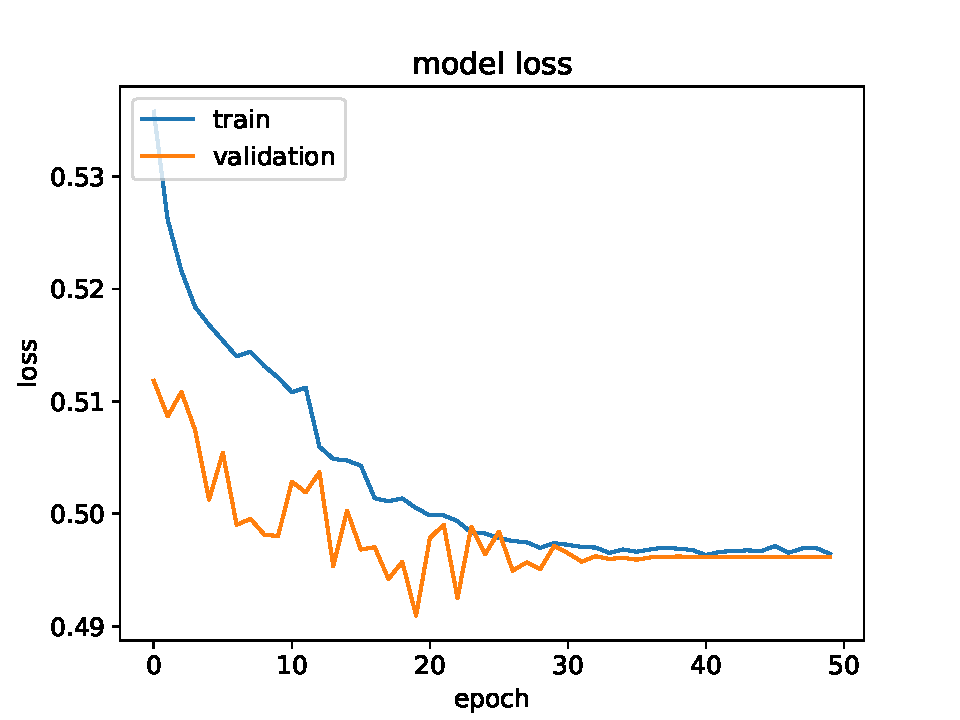
\includegraphics[scale=.75]{assets/chap04/model_loss.pdf}
    \caption{The training process of the classifier for top quark reconstruction, which fully converged after about 35 epochs.}
    \label{fig:ch_4_loss}
\end{figure}

As mentioned previously, the Monte Carlo simulations are provided in the ROOT file format. These are converted in the \emph{DataFrame} data structure, which provides simpler access and manipulation of numerical tables, and is implemented by \emph{pandas}, a Python software library for data manipulation and analysis. The data from the electron and muon channel were then merged together in a single large \emph{DataFrame} object. Then they were preprocessed and the values for input variables were extracted, as outlined in detail in Section \ref{sec:ch-4-input-vars}, and used to train the classifier.

The classifier was trained in mini-batch mode on \num{344374} samples and validated on \num{114792} samples, i.e. \SI{75}{\%} of the data was used for training, \SI{25}{\%} for validation. The batch size was selected to be 256: the algorithm takes the first 256 samples from the \num{344374} samples and trains the network, next it takes the second 256 samples, trains the network again and repeats the procedure until all samples have propagated through the network. After each propagation, the network's parameters are updated, in this case the parameters were updated \num{1346} times. This makes the network converge faster, as its weights are updated more often than in the case of one single large batch \cite{153535}. This is repeated for every training epoch with the batch data being shuffled every time.

The selection of the batch size is also crucial for the discriminatory power of the classifier: a small batch may negatively impact the accuracy of gradient estimation, i.e. the direction of the gradient may fluctuate much more often than for larger batches. During the trainings made in the scope of this work, smaller batch sizes lead to considerably longer training times, better AUC-ROC scores, but worse top quark reconstruction accuracy.

The training time of the classifier was about 20 minutes -- the history of the loss value is shown in Figure \ref{fig:ch_4_loss} -- with the classifier converging around the 35th epoch.

Appendix \ref{ch:appendix_a} lists the input variables for which the best improvements in descending order in top quark reconstruction were achieved.

Appendix \ref{ch:appendix_lr} plots different average learning rates that were tried during training and their impact on top quark reconstruction improvement --- the average learning rate depends on the initial learning rate of the Adam optimizer and the learning rate reduction factor --- the logarithmic learning rate that yields the best improvement appears to be in the $10^{-6}$ order of magnitude.

\section{Evaluation}
\label{sec:ch-4-eval}
What follows is an evaluation of the trained classifier model using the ROC curve and the improvement comparison over the best-mass method.

After the classifier was trained, two ROC curves with training and test data respectively were plotted (Figure \ref{fig:ch_4_roc}). The test data set consisted of \num{475476} events, as opposed to \num{459166} events of the training data set mentioned previously. Both ROC curves differ very little in their progression and values, which is confirmation that the neural network model was not overtrained. The ROC-AUC score for the test data case was 0.823.

Next, a comparison of the classifier against the best-mass method was made in how accurately they each identify the jet that originated from the top quark. The test data set with \num{475476} events was used. The best-mass method accurately predicted the jet in \SI{70.07}{\%} of the events, the classifier in \SI{77.90}{\%}, an improvement of \SI{7.83}{\%} over the best-mass method.

\begin{figure}[h]
    \centering
    \begin{subfigure}{0.5\textwidth}
        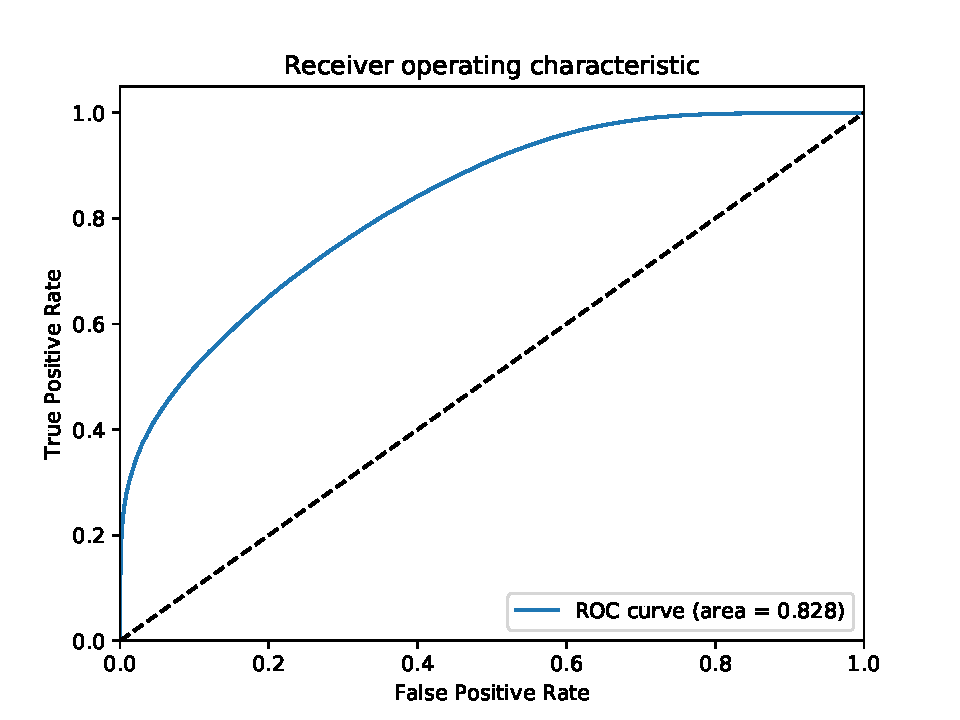
\includegraphics[scale=.6]{assets/chap04/roc_train.pdf}
        \caption{Using training data}
        \label{fig:ch_4_roc_train}
    \end{subfigure}
    
    \begin{subfigure}{0.5\textwidth}
        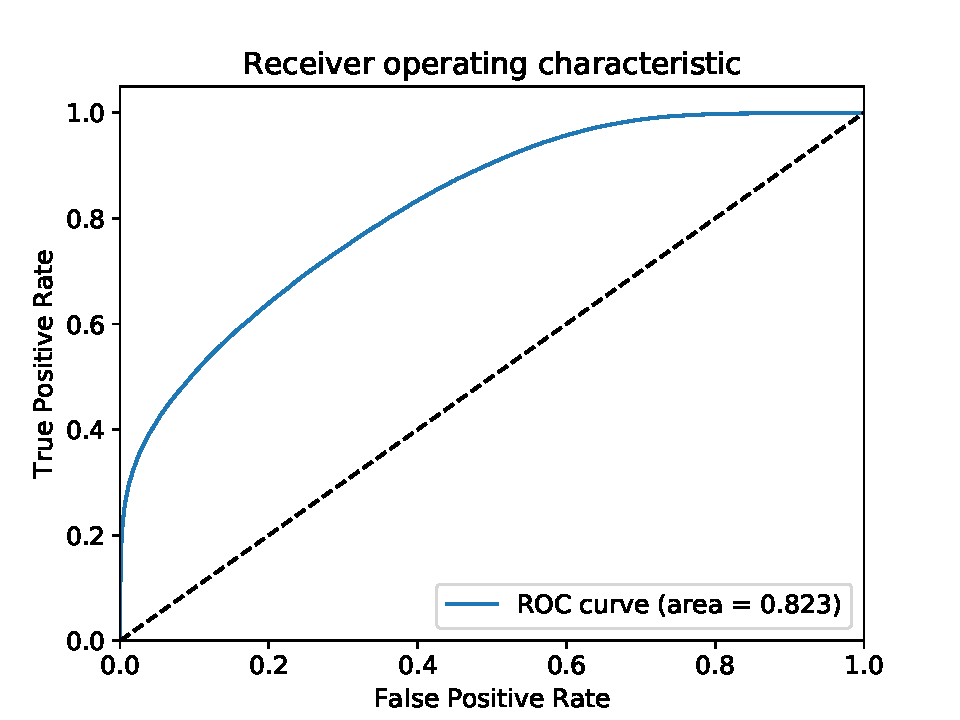
\includegraphics[scale=.6]{assets/chap04/roc_test.pdf}
        \caption{Using test data}
        \label{fig:ch_4_roc_test}
    \end{subfigure}
    \caption{ROC curve for classifier evaluation.}
    \label{fig:ch_4_roc}
\end{figure}